% \documentclass[sigconf]{acmart}
% \documentclass[sigconf, authordraft]{acmart}
% \usepackage{longtable}
% \usepackage{subcaption}
% \usepackage{amsmath}

%%
%% This is file `sample-manuscript.tex',
%% generated with the docstrip utility.
%%
%% The original source files were:
%%
%% samples.dtx  (with options: `manuscript')
%% 
%% IMPORTANT NOTICE:
%% 
%% For the copyright see the source file.
%% 
%% Any modified versions of this file must be renamed
%% with new filenames distinct from sample-manuscript.tex.
%% 
%% For distribution of the original source see the terms
%% for copying and modification in the file samples.dtx.
%% 
%% This generated file may be distributed as long as the
%% original source files, as listed above, are part of the
%% same distribution. (The sources need not necessarily be
%% in the same archive or directory.)
%%
%% Commands for TeXCount
%TC:macro \cite [option:text,text]
%TC:macro \citep [option:text,text]
%TC:macro \citet [option:text,text]
%TC:envir table 0 1
%TC:envir table* 0 1
%TC:envir tabular [ignore] word
%TC:envir displaymath 0 word
%TC:envir math 0 word
%TC:envir comment 0 0
%%
%%
%% The first command in your LaTeX source must be the \documentclass command.
%%%% Small single column format, used for CIE, CSUR, DTRAP, JACM, JDIQ, JEA, JERIC, JETC, PACMCGIT, TAAS, TACCESS, TACO, TALG, TALLIP (formerly TALIP), TCPS, TDSCI, TEAC, TECS, TELO, THRI, TIIS, TIOT, TISSEC, TIST, TKDD, TMIS, TOCE, TOCHI, TOCL, TOCS, TOCT, TODAES, TODS, TOIS, TOIT, TOMACS, TOMM (formerly TOMCCAP), TOMPECS, TOMS, TOPC, TOPLAS, TOPS, TOS, TOSEM, TOSN, TQC, TRETS, TSAS, TSC, TSLP, TWEB.
% \documentclass[acmsmall]{acmart}

%%%% Large single column format, used for IMWUT, JOCCH, PACMPL, POMACS, TAP, PACMHCI
% \documentclass[acmlarge,screen]{acmart}

%%%% Large double column format, used for TOG
% \documentclass[acmtog, authorversion]{acmart}

%%%% Generic manuscript mode, required for submission
%%%% and peer review
\documentclass[sigconf]{acmart}

\usepackage{longtable}
\usepackage{subcaption}
\usepackage{amsmath}

%% Fonts used in the template cannot be substituted; margin 
%% adjustments are not allowed.
%%
%% \BibTeX command to typeset BibTeX logo in the docs
\AtBeginDocument{%
  \providecommand\BibTeX{{%
    \normalfont B\kern-0.5em{\scshape i\kern-0.25em b}\kern-0.8em\TeX}}}

%% Rights management information.  This information is sent to you
%% when you complete the rights form.  These commands have SAMPLE
%% values in them; it is your responsibility as an author to replace
%% the commands and values with those provided to you when you
%% complete the rights form.
\setcopyright{acmcopyright}
\copyrightyear{2018}
\acmYear{2018}
\acmDOI{XXXXXXX.XXXXXXX}

%% These commands are for a PROCEEDINGS abstract or paper.
\acmConference[Conference acronym 'XX]{Make sure to enter the correct
  conference title from your rights confirmation emai}{June 03--05,
  2018}{Woodstock, NY}
%
%  Uncomment \acmBooktitle if th title of the proceedings is different
%  from ``Proceedings of ...''!
%
\acmBooktitle{Woodstock '18: ACM Symposium on Neural Gaze Detection,
 June 03--05, 2018, Woodstock, NY} 
\acmPrice{15.00}
\acmISBN{978-1-4503-XXXX-X/18/06}


%%
%% Submission ID.
%% Use this when submitting an article to a sponsored event. You'll
%% receive a unique submission ID from the organizers
%% of the event, and this ID should be used as the parameter to this command.
%%\acmSubmissionID{123-A56-BU3}

%%
%% For managing citations, it is recommended to use bibliography
%% files in BibTeX format.
%%
%% You can then either use BibTeX with the ACM-Reference-Format style,
%% or BibLaTeX with the acmnumeric or acmauthoryear sytles, that include
%% support for advanced citation of software artefact from the
%% biblatex-software package, also separately available on CTAN.
%%
%% Look at the sample-*-biblatex.tex files for templates showcasing
%% the biblatex styles.
%%

%%
%% The majority of ACM publications use numbered citations and
%% references.  The command \citestyle{authoryear} switches to the
%% "author year" style.
%%
%% If you are preparing content for an event
%% sponsored by ACM SIGGRAPH, you must use the "author year" style of
%% citations and references.
%% Uncommenting
%% the next command will enable that style.
%%\citestyle{acmauthoryear}

%%
%% end of the preamble, start of the body of the document source.
\begin{document}

%%
%% The "title" command has an optional parameter,
%% allowing the author to define a "short title" to be used in page headers.
% \title{The Name of the Title is Hope}

% %%
% %% The "author" command and its associated commands are used to define
% %% the authors and their affiliations.
% %% Of note is the shared affiliation of the first two authors, and the
% %% "authornote" and "authornotemark" commands
% %% used to denote shared contribution to the research.
% \author{Ben Trovato}
% \authornote{Both authors contributed equally to this research.}
% \email{trovato@corporation.com}
% \orcid{1234-5678-9012}
% \author{G.K.M. Tobin}
% \authornotemark[1]
% \email{webmaster@marysville-ohio.com}
% \affiliation{%
%   \institution{Institute for Clarity in Documentation}
%   \streetaddress{P.O. Box 1212}
%   \city{Dublin}
%   \state{Ohio}
%   \country{USA}
%   \postcode{43017-6221}
% }

\hypertarget{abstract}{%
\section{Abstract}\label{abstract}}

Natural cooling, utilizing non-mechanical cooling, presents a low-carbon
and low-cost way to provide thermal comfort in residential buildings.
However, designing naturally cooled buildings requires a clear
understanding of how opening and closing windows affect occupants'
comfort. Predicting when and why occupants open windows is a challenging
task, often relying on specialized sensors and building-specific
training data. This limits the scalability of natural cooling solutions.
Here, we propose a novel unsupervised method that utilizes easily
deployable off-the-shelf temperature and humidity sensors to detect
window operations. The effectiveness of our approach is evaluated using
an empirical dataset and compared with a state-of-the-art support vector
machine (SVM) model. The results demonstrate that our proposed method
outperforms the SVM on key indicators, except when indoor and outdoor
temperatures have small differences. Unlike the SVM's sensitivity to
time series characteristics, our proposed method relies solely on indoor
temperature and exhibits robust performance in pilot studies, making it
a promising candidate for developing a highly scalable and generalizable
window operation detection model. This work demonstrates the potential
of unsupervised data-driven methods for understanding window operations
in residential buildings. By enabling more accurate modeling of
naturally cooled buildings, our work aims to facilitate the widespread
adoption of this low-cost and low-carbon technology.

\hypertarget{introduction}{%
\section{Introduction}\label{introduction}}

\hypertarget{literature-review}{%
\section{Literature Review}\label{literature-review}}

Several research studies have been performed to detect window
opening/closing actions in the past. Environmental parameters such as
indoor and outdoor temperature, relative humidity, wind speeds, solar
radiation, etc. have been widely investigated, and numerous studies have
found window operation to be affected primarily by these factors. Almost
all of these studies have considered indoor and outdoor temperatures and
deemed them to be significant. Data-driven machine learning models have
been employed to predict these dynamic window actions taken by the
users. These models predict the probability of either the window state
(i.e.~open or close) or a certain action being taken (opening or closing
a window). Supervised ML models such as Logistic regression and Markov
chain models, followed by artificial neural networks, have been heavily
relied upon to study the probabilistic correlation between the window
state and explanatory variables monitored. Other ML models such as
support vector machines, and random forest classifiers have been
explored in more recent studies to predict window-opening behavior based
on both environmental and contextual features. However, these supervised
models often rely on labeled long-term data collection, usually spanning
over 6 months or multiple seasons. They suffer from a lack of
generalizability as their results have to be specifically tuned for the
context in which data was collected, either constrained by building type
or climate. This makes them ineffective tools for scaling natural
cooling to a large number of buildings.

Additionally, while environmental parameters, for eg, air temperature
and relative humidity are commonly used, sensors to monitor window
opening actions are relatively difficult to install and could be
intrusive for building occupants. Therefore, we propose a novel
unsupervised window opening and closing detection method that utilizes
easy to deploy off-the-shelf temperature and humidity sensors.

As window operation detection is commonly a binary classification task
in machine learning, several metrics have been used to assess the
prediction performance of window status. These evaluation metrics,
frequently referred to in literature are overall accuracy of the model,
precision, recall, f-1 score, coefficient of determination (R\^{}2),
mean average error (MAE), and root mean square error (RMSE). R\^{}2,
MAE, and RMSE are typically used when the output of model is numeric
such as the probability of the action being taken. Otherwise, the
ability to correctly estimate the window state (open or close) is
normally assessed by accuracy, precision, recall, and f-1 scores. Some
domain specific metrics for evaluating the prediction performance of the
window open/close classification task have also been proposed in
previous studies in order to investigate the overall accuracy of the
model as well as the consistency of true estimates for window states.
These include ratio of total window opening time over total monitoring
period, number of actions taken, and median opening/closing durations.
Recently, de Rautlin et al.~proposed domain oriented metrics to improve
coherence of results such as number of true and false openings, total
time of true and false openings, and average true opening accuracy score
-\textgreater{} we will discuss in more detail further in the paper, as
we will evaluate our model based on these metrics, in addition to, our
developed custom metrics.

\hypertarget{methods}{%
\section{Methods}\label{methods}}

In this section, we descibe our data collection process, the two window
detection algorithms we examined, and the metrics we used to evaluate
these algorithms.

\hypertarget{data-collection}{%
\subsection{Data Collection}\label{data-collection}}

We collected data for short periods of time over three months in the
summer. We placed HOBO® Temp-RH 2.5\% Data Logger (UX100-011) (CITE)
sensors in two adjacent rooms in a multi-family residential building,
and measured indoor temperatures, \(T_{meas}(t)\) and relative humidity,
\(RH_{meas}(t)\). In hopes of capturing the average room temperature,
sensors were intentionaly positioned away from drafts that could come in
through windows (CITE Huang). We also collected data on the ambient
temperature, \(T_{amb}(t)\) and relative humidity \(RH_{amb}(t)\) from a
local weather station (CITE). In one room, the window state, \(W(t)\),
was held constant. In the adjacent room, window state was allowed to
vary between open and closed.

Descriptions of the data in the rooms where the window state varied are
provided in Table~\ref{tbl-data-collected}. The experiments are labeled
as experiments A, B, and C, corresponding to data recorded at the
beginning on July 20, July 27, and September 8 respectively. Experiment
B was much longer than the other experiments, spanning 14 days. Data for
experiments A and C were collected for less than 4 days. The window was
open for 5 percent of time recorded time in experiment B, which is
shorter than the the 20 percent or greater recorded for other
experiments (FIX).

\hypertarget{tbl-data-collected}{}
\begin{longtable}[]{@{}llll@{}}
\caption{\label{tbl-data-collected}Data Collected}\tabularnewline
\toprule()
& A & B & C \\
\midrule()
\endfirsthead
\toprule()
& A & B & C \\
\midrule()
\endhead
Starting Day & Jul 20 & Jul 27 & Sep 08 \\
Data Length & 4 days & 14 days & 3 days \\
Room & 1 & 0 & 0 \\
Opening Percentage & 41.3 & 5.2 & 22.1 \\
\bottomrule()
\end{longtable}

To develop an understanding of how the indoor and ambient quantities of
interest changed across the different experiments, we examined the
distributions of the data. The internal relative humidity was higher
than the ambient relative humidity across experiments. The temperature
distributions, which had distinctive fluctiations across experiments,
are shown in Figure~\ref{fig-data-collected}. We observe that experiment
B had the widest distribution of indoor temperatures. Experiment C had
internal temperatures that were higher and closer to the mean of the
ambient temperatures. This can be attributed to higher ambient
temperatures that were recorded during this time period, which makes for
a particularly interesting edge case. (FIX: the difference in
distributions is a bit hard to see with the narrow subplots, consider
horizontal layout)

\begin{figure}

\begin{minipage}[t]{0.33\linewidth}

{\centering 

\raisebox{-\height}{

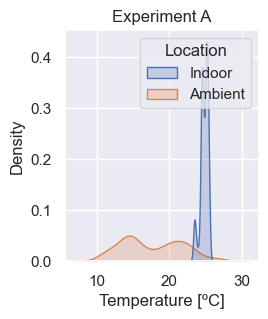
\includegraphics{figs/dist_expa.png}

}

}

\subcaption{\label{fig-dexpa}}
\end{minipage}%
%
\begin{minipage}[t]{0.33\linewidth}

{\centering 

\raisebox{-\height}{

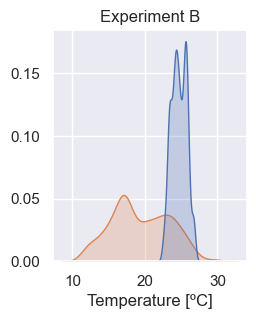
\includegraphics{figs/dist_expb.png}

}

}

\subcaption{\label{fig-dexpb}}
\end{minipage}%
%
\begin{minipage}[t]{0.33\linewidth}

{\centering 

\raisebox{-\height}{

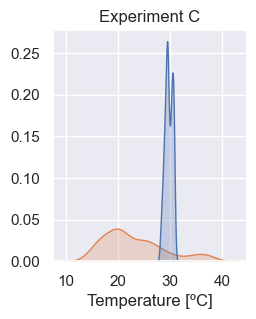
\includegraphics{figs/dist_expc.png}

}

}

\subcaption{\label{fig-dexpc}}
\end{minipage}%

\caption{\label{fig-data-collected}Distributions of temperature across
experiments}

\end{figure}

In summary, the three receorded datasets present various degrees of
difficulty for a detection algorithm. Experiment A presents the most
favorable case for window state detection, as it has a fairly even
amount of opening and closed states, as well as distinct indoor and
ambient measured temperatures and relative humidities. Although
experiment B also has noteable distinctions in terms of temperature and
relative humidity, the window states are extremely unbalanced.
Experiment C has both unbalanced window states and little distincition
between indoor and outdoor temperature.

\hypertarget{detection-methods}{%
\subsection{Detection Methods}\label{detection-methods}}

In the following section, we discuss the two methods that were used to
detect window state changes. The first is a smoothing technique (ST)
that we have developed, and the second is a machine learning method that
has been studied in the literature (CITE).

\hypertarget{new-method-smoothing-technique}{%
\subsubsection{New Method: Smoothing
Technique}\label{new-method-smoothing-technique}}

Our approach relies on an intuitive understanding of window operation
detection. We expect a typical time series recording of a quantity of
interest, in this case the measured indoor temperature, \(T_{meas}(t)\),
to contain information that reflects the seasonality of ambient
quantities, noise due to occurrences within the space where measurements
are being taken, and the desired signal of changes in window state. The
way in which these three components of a measurement are combined is
unknown, and, the noise component in particular cannot be known based on
the measurements we have collected. As we have recorded information
about the ambient temperature, \(T_{amb}(t)\), we focus on removing the
seasonality from \(T_{meas}(t)\), hypothesizing that this will reveal
the window state signal and noise. An optimal technique will additinally
isolate the window state signal from the unknown noise.

To remove the seasonality from the measured data, we examined three
methods of de-seasonalizing: using sinusoidal fit, using an
exponentially weighted mean function, and using a
seasonal-trend-decomposition (CITE all), which consists of optimizing
the parameters of a sine function to fit a specific time series, purely
reflects seasonality. However, this does not nessecarily account for the
seasonality that \(T_{meas}(t)\) experiences due to changes in outdoor
temperature. The exponentially weighted mean function is simply a moving
average of the indoor temperature signal -- it captures some seasnality
and some noise. The seasonal component of a seasonal trend decomposition
represents a middle ground. In preliminary studies, we found that the
exponentially weighted mean function performed the best in isolating
window detection, which follows from our intuition that both the
seasonal components and noise need to be isolated.

ST proceeds as follows. The goal is to identify \(W(t)\), window state
as a function of time. This can take on two values: 0, representing
window closed, or 1, representing window open. We have an observed
variable \(T(t) = T_{meas}(t)\), which represents the measurement of the
indoor temperature. We apply an exponentially weighted mean (EWM)
function to \(T(t)\), creating a smoothed time series,
\(\overline{T(t)}\), which ideally removes strong peaks that would
reflect changes in window state, and isolates information concerning the
seasonal response and additional noise. This technique operates under
the assumption that the instantaneous change in indoor temperature due
to window opening is greater than any other potential source of
instantaneous temperature change. In reality, other unknown occurences
within a room might cause large temperature spikes, which would
interfere with the efficacy of \(\overline{T(t)}\). Subtracting
\(\overline{T(t)}\) from \(T(t)\) yields \(T'(t)\), which is a time
series that reflects changes in the window state and some additional
noise.

In order to confidently identify the where the changes in window state
occur, we examine the first and second derivatives of \(T'(t)\),
\(\frac{dT'(t)}{dt}\) and \(\frac{d^2T'(t)}{dt^2}\). The second
derivative is particularly effective for identifying change points. In
order to predict where window changes occur, we apply a principles from
statistical hypothesis testing. We assume that the time series
\(\frac{d^2T'(t)}{dt^2}\) is normally distributed. Therefore, any value
in \(\frac{d^2T'(t)}{dt^2}\) that is more than 2 standard deviations
away from the mean of this time series is unlikely to occur, and could
possibly indicate an instance of a change in window state. We will use
these unlikely values as initial guesses \(G(t)\). They take on positive
or negative values depending on whether they are predicting a transition
from window open to close, or window close to open. Therefore, we round
the values of \(G(t)\) to 0 or 1 to reflect this. Finally, we
interpolate between the rounded values of \(G(t)\), so that we only
predict a change in window state when \(G(t)\) transitions between 0 and
1. This prediction of the window state is called \(I(t)\).

\hypertarget{machine-learning-method-support-vector-machine}{%
\subsubsection{Machine Learning Method: Support Vector
Machine}\label{machine-learning-method-support-vector-machine}}

We used a separate method in order to compare the efficacy of ST that we
developed. We chose to use an SVM, as it has been shown in literature
(CITE de Rautlin de Roy) to have robust performance across a wide range
of features. SVMs are straightforward to implement with relatively few
hyper-parameters, as compared to other methods that have been recently
shown to have high performance on the window detection problem. For our
particular interest in unsupervised problems, the availability of an
unsupervied implementation of a SVM through sklearn's One-Class SVM is
also ideal (CITE).

In a similar way to a linear regression, SVMs approximate a line of best
fit using the features and labels provided. However, with the use of
kernel functions that can map high dimensional feature spaces to ones of
lower dimensions, SVMs also effectively create hyperplanes of best fit
in order to classify datasets. The use of a kernel function also enables
the introduction of mappings that may be a better suited to the
structure of features in a given dataset (CITE).

Our focus was trying to get the best performance from the SVM using an
optimal set of features with optimal pre-processing functions applied.
We therefore came up with combinations of the various features we had
access to, as well as their derivatives and differences from one
another. The base features were: ambient temperature \(T_{amb}(t)\),
measured temperature \(T_{meas}(t)\), and their derivatives,
\(\frac{\mathrm{d}}{\mathrm{d}t}T_{meas}\) and
\(\frac{\mathrm{d}}{\mathrm{d}t}T_{amb}\). We also considered the
difference between ambient temperature and measured temperature
\(T_{amb} - T_{meas}\) , the difference between measured temperature and
the derivative of measured temperature,
\(T_{meas} - \frac{\mathrm{d}}{\mathrm{d}t}T_{meas}\). We also had the
same features for relative humidity. After creating combinations of
these base features, we had a test set of 113 combinations.

For each experiment we recorded data for, we created an SVM for each of
the combinations in the test set, which resulted in 3x113 different SVM
models. We chose not to perform hyperparameter tuning for the SVMs, and
used the default parameters defined by sklearn which consists of a
radial basis function kernel. As mentioned above, we are interested in
the developing an unsupervised detection method. Therefore, we used the
One-Class SVM implementation which is ideal for anomally detection.
Outliers are identified by clustering features to create the hyperplanes
for classification.

The SVM approach differs from ST that we have developed, and is similar
to other window techniques in that it is a highly generalizable method
that is not developed with window detection in mind. A wide array of
input features can be tested in order to get an acceptable prediction
accuracy. However, this might not be acceptable in practice, as
different scenarios or window operation behaviors, will demand different
sets of input features. In the event the true window detection pattern
is unknown, it will be difficult to know which input features are giving
a trustworthy result.

\hypertarget{evaluation-metrics}{%
\subsection{Evaluation Metrics}\label{evaluation-metrics}}

We used 3 sets of metics to evaluate the methods we chose. The first two
sets follow from a recent paper that compared the efficacy of different
machine learning algorithms for window detection(CITE) , and the final
set of metrics were developed to more closely examine specific behavior
of chosen models.

\hypertarget{standard-metrics}{%
\subsubsection{Standard Metrics}\label{standard-metrics}}

\textbf{Macro average F-1 score}: The F-1 score is a classic metric for
evaluating the performance of classification algorithms. It it condenses
information about the precision of a model in predicting a certain
class, as well as its ability to recall the the available data. The
macro averaged F-1 score averages the F-1 scores for all individual
classes, but does not introduce weights in the averaging to reflect that
the classes may be unbalanced. As shown in
Table~\ref{tbl-data-collected}, the data sets we have very from fairly
balanced in experiment A, to highly unbalanced in experiment B.
Therefore, using the macro average F-1 score provides a worst case
performance. Using this F1-score also provides a basis of comparison to
(CITE) . The implementation for computing this metric comes from scikit
learns classification report (CITE).

\hypertarget{de-rautlin-de-roy-metrics}{%
\subsubsection{De Rautlin de Roy
Metrics}\label{de-rautlin-de-roy-metrics}}

The following metrics were introduced by (CITE), and represent window
detection specific evaluation metrics.

\textbf{Opening Accuracy}: The opening accuracy is an average of scores
given to each opening instance predicted by a window detection model. An
opening instance is an interval on \(t\), such as
\(t_{nk} = t_n, t_{n+1}, \dots , t_k\), where the final guess from the
algorithm, \(I(t_{nk}) = 1\). An opening receives a score of 0 if it
does not correspond to a a true opening:
\(I(t_{nk}) = 1, W(t_{nk} = 0)\), and a score of 1 it perfectly
corresponds to a true opening: \(I(t_{nk}) = 1, W(t_{nk} = 1)\). The
score for a given predicted opening interval decreases by a penalty of
0.33 for each time step that does not align to a true opening.
Therefore, a predicted opening interval \(I(t_{nk}) = 1\) that aligns a
true opening interval will have a score of at most 0 if it extends for
more than two times steps away from a true value. For the opening
accuracy metric desciribed by (CITE drdr), the value for each opening
interval are bounded at 0, and then are averaged to get the opening
accuracy for an entire model. Here we also consider an unbounded opening
accuracy where the score for a given interval is not bounded at 0 but is
allowed to become negative. This unbounded metric provides clearer
indication of how ``off'' models are, given that due to the unfavorable
nature of some of the datasets collected, many models we examined
actually had a bounded opening accuracy of 0.

\textbf{True or False Opening Time}: This true opening time reflects the
total amount of time when \(I(t) = W(t) = 1\). False opening times occur
when \(I(t) = 1, W(t) = 0\). The metric is somewhat similar to the F-1
score in that rather than looking at specifically at change points, it
provides information the entire time period.

\hypertarget{custom-metrics}{%
\subsubsection{Custom Metrics}\label{custom-metrics}}

We developed the final set of metrics based on the intuition that if a
model is perfectly able to capture the specific times when a window
state changes, then it is performing extremely well. We classify a
``guess'', as any value of \(I(t)\), and an ``action'' as any value of
\(W(t)\). A ``hit'' occurs when \(I(t) = W(t)\). Like (CITE) we consider
a prediction accurate if it is withing at most 2 timestamps of the true
occurrence. Therefore, a ``near hit'' occurs when \(I(t) = W(t \pm 2)\).
The metrics we examine are given below.

\textbf{Hits + Near Hits Over Guesses}: This metric accounts for the
variability in guesses. A ratio of 1 indicates that all guesses taken by
the model were accurate within two timestamps. A ratio close to 0
indicates that a lot of guesses were taken, but relatively few were
close to where change occurred in the true window state.

\textbf{Guesses Over Actions}: This metric implicitly accounts for the
ability of the model to capture the pattern of the changes in window
state. If the true window state changed only 10 times, but the model
predicts changes on the order of 100, then the model is performing
poorly. A perfect score is 1.

\hypertarget{results}{%
\section{Results}\label{results}}

\begin{figure}

\begin{minipage}[t]{0.33\linewidth}

{\centering 

\raisebox{-\height}{

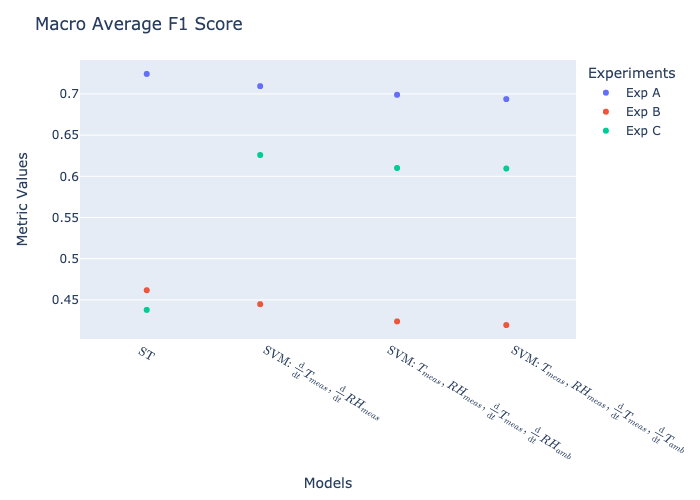
\includegraphics{figs/f1.png}

}

}

\subcaption{\label{fig-f1}}
\end{minipage}%
%
\begin{minipage}[t]{0.33\linewidth}

{\centering 

\raisebox{-\height}{

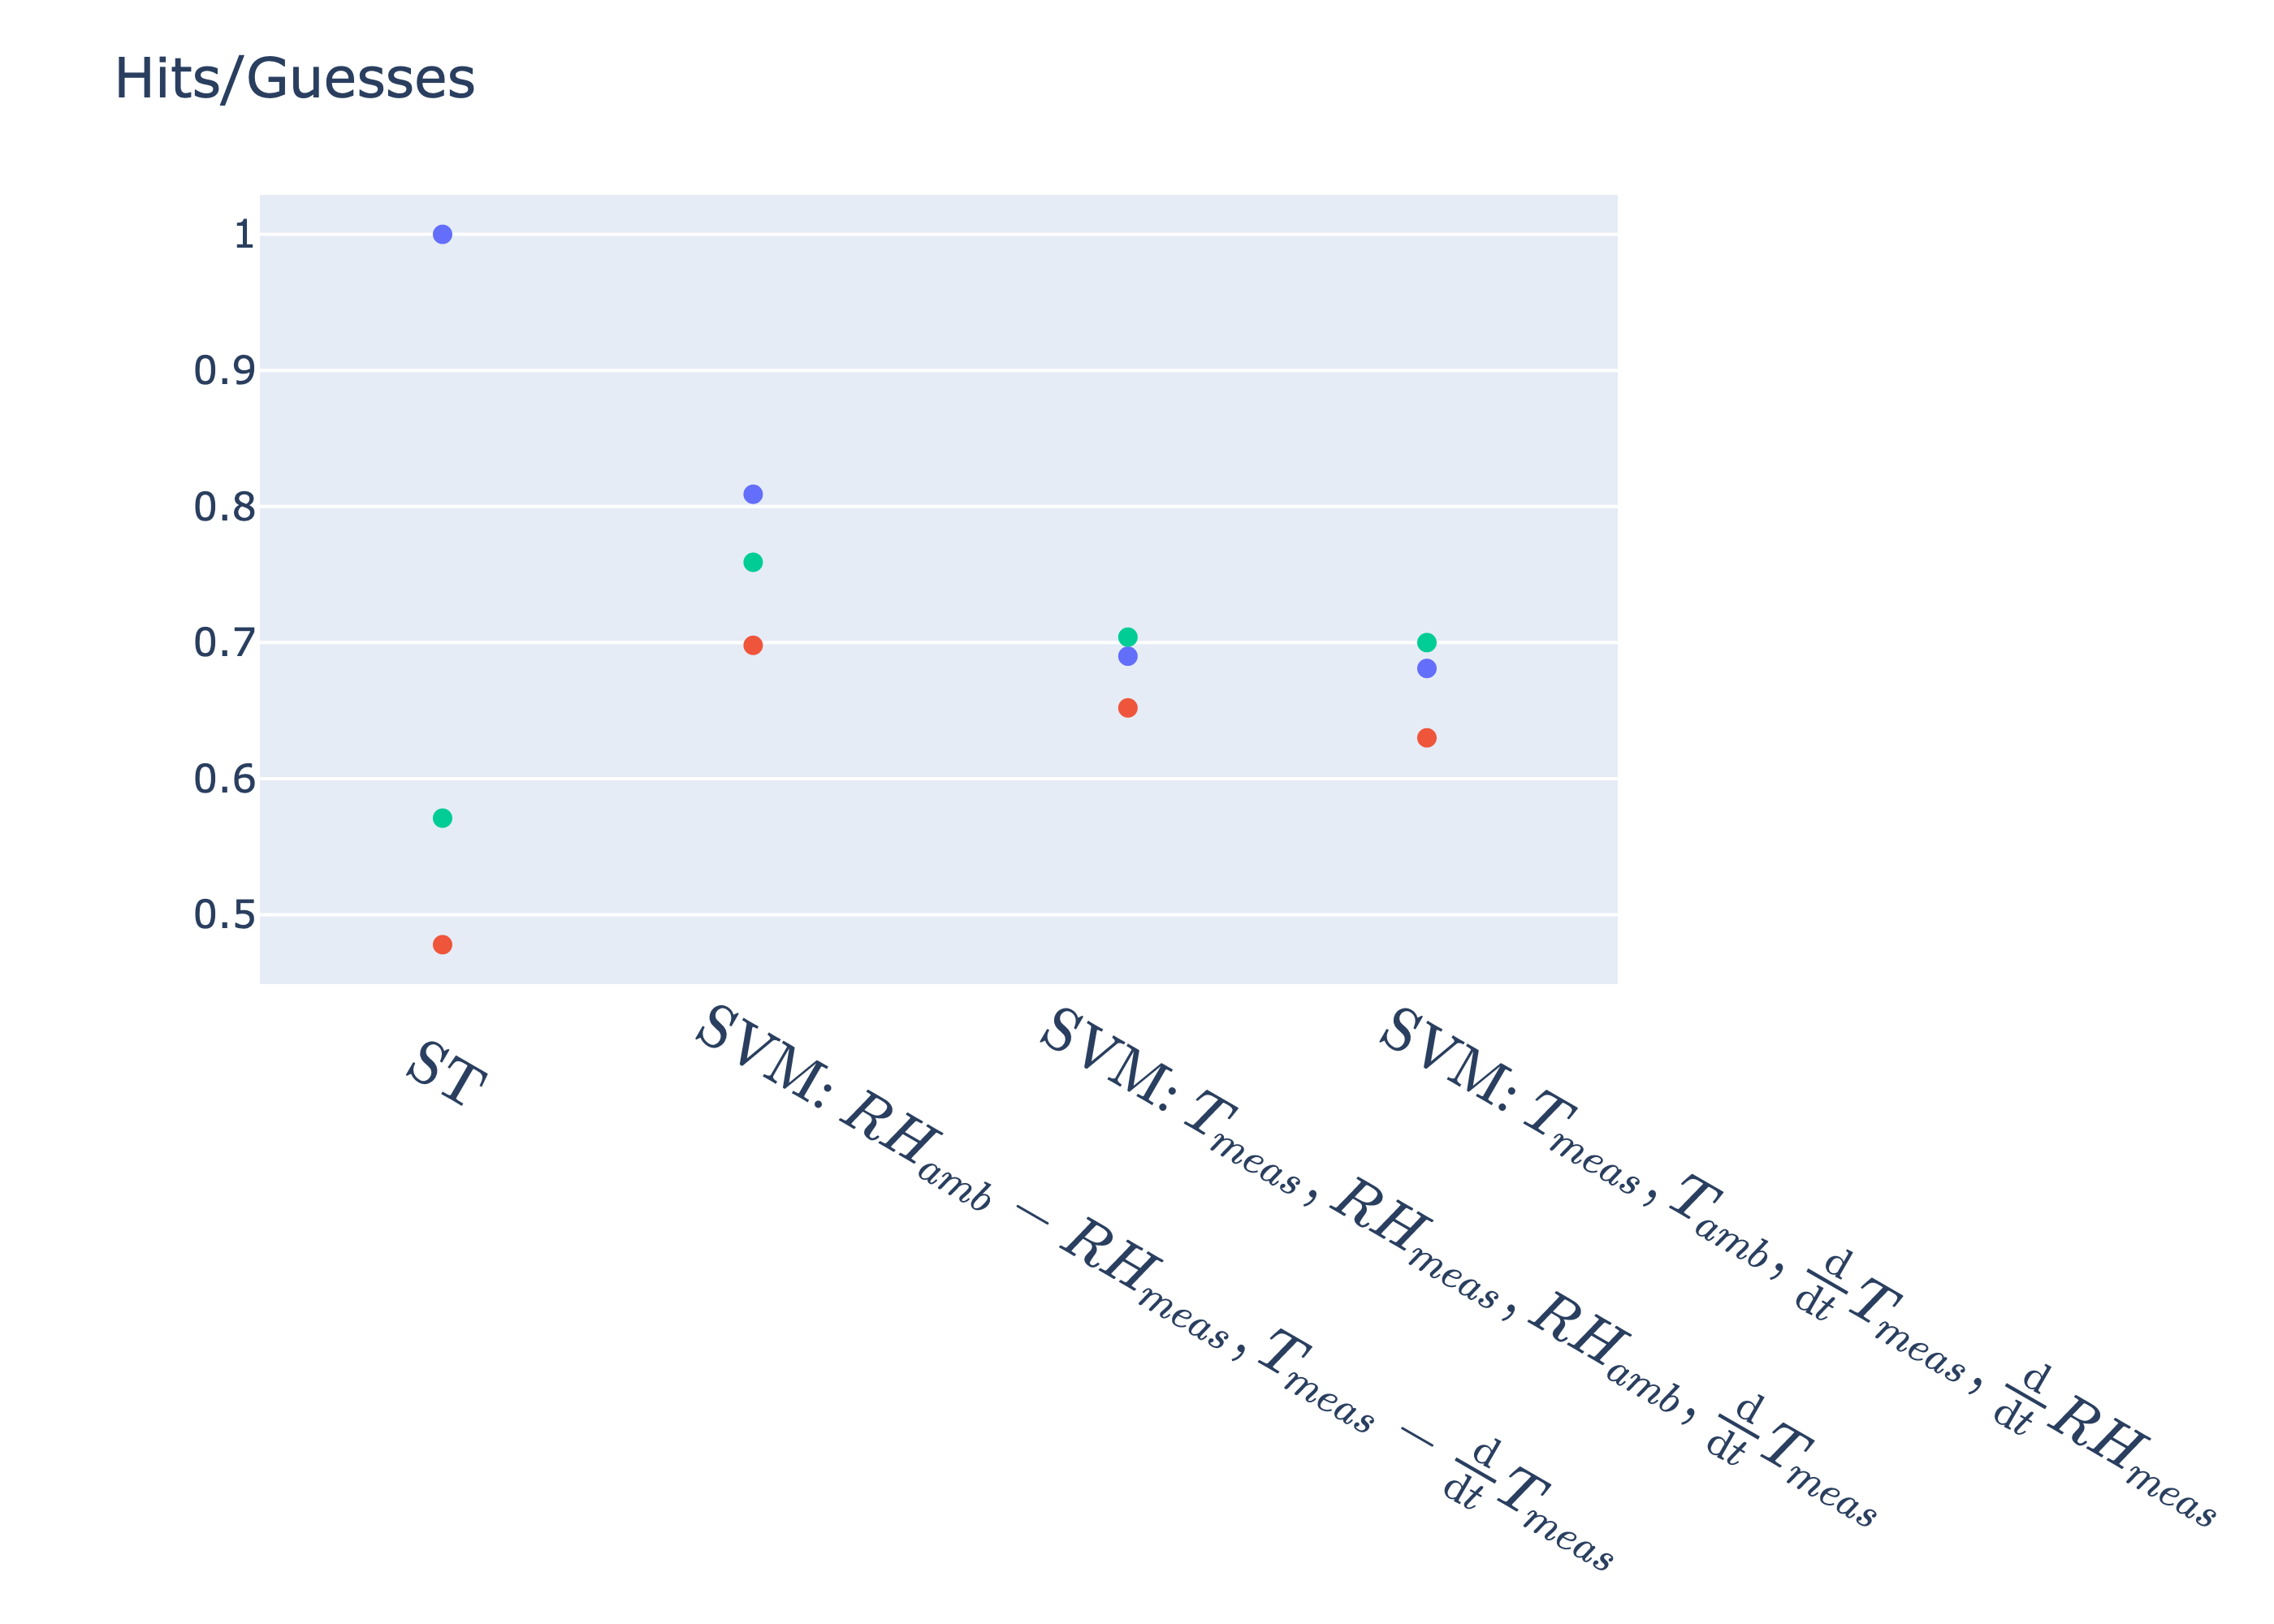
\includegraphics{figs/hits_guesses_ratio.png}

}

}

\subcaption{\label{fig-hg}}
\end{minipage}%
%
\begin{minipage}[t]{0.33\linewidth}

{\centering 

\raisebox{-\height}{

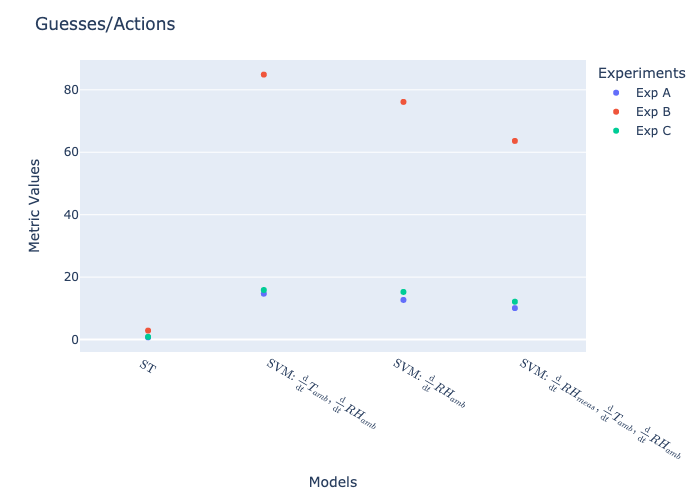
\includegraphics{figs/guesses_actions_ratio.png}

}

}

\subcaption{\label{fig-ga}}
\end{minipage}%
\newline
\begin{minipage}[t]{0.33\linewidth}

{\centering 

\raisebox{-\height}{

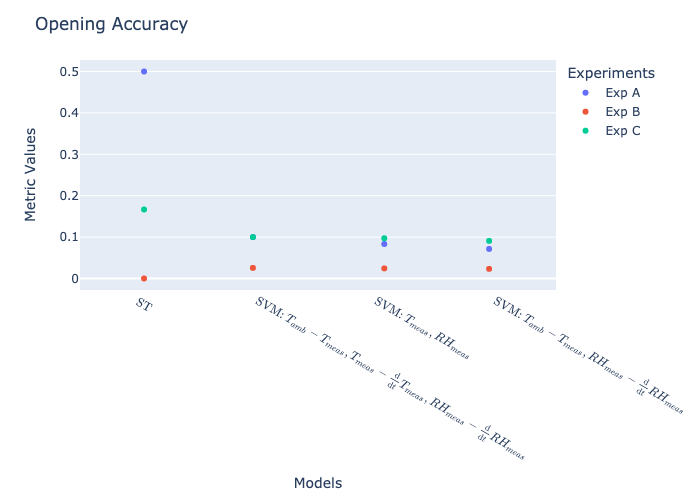
\includegraphics{figs/opening_acc.png}

}

}

\subcaption{\label{fig-oa}}
\end{minipage}%
%
\begin{minipage}[t]{0.33\linewidth}

{\centering 

\raisebox{-\height}{

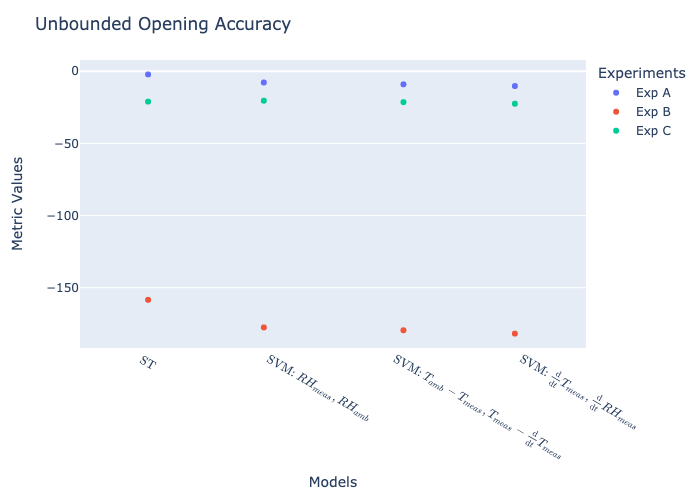
\includegraphics{figs/unbounded_opening_acc.png}

}

}

\subcaption{\label{fig-uoa}}
\end{minipage}%
%
\begin{minipage}[t]{0.33\linewidth}

{\centering 

\raisebox{-\height}{

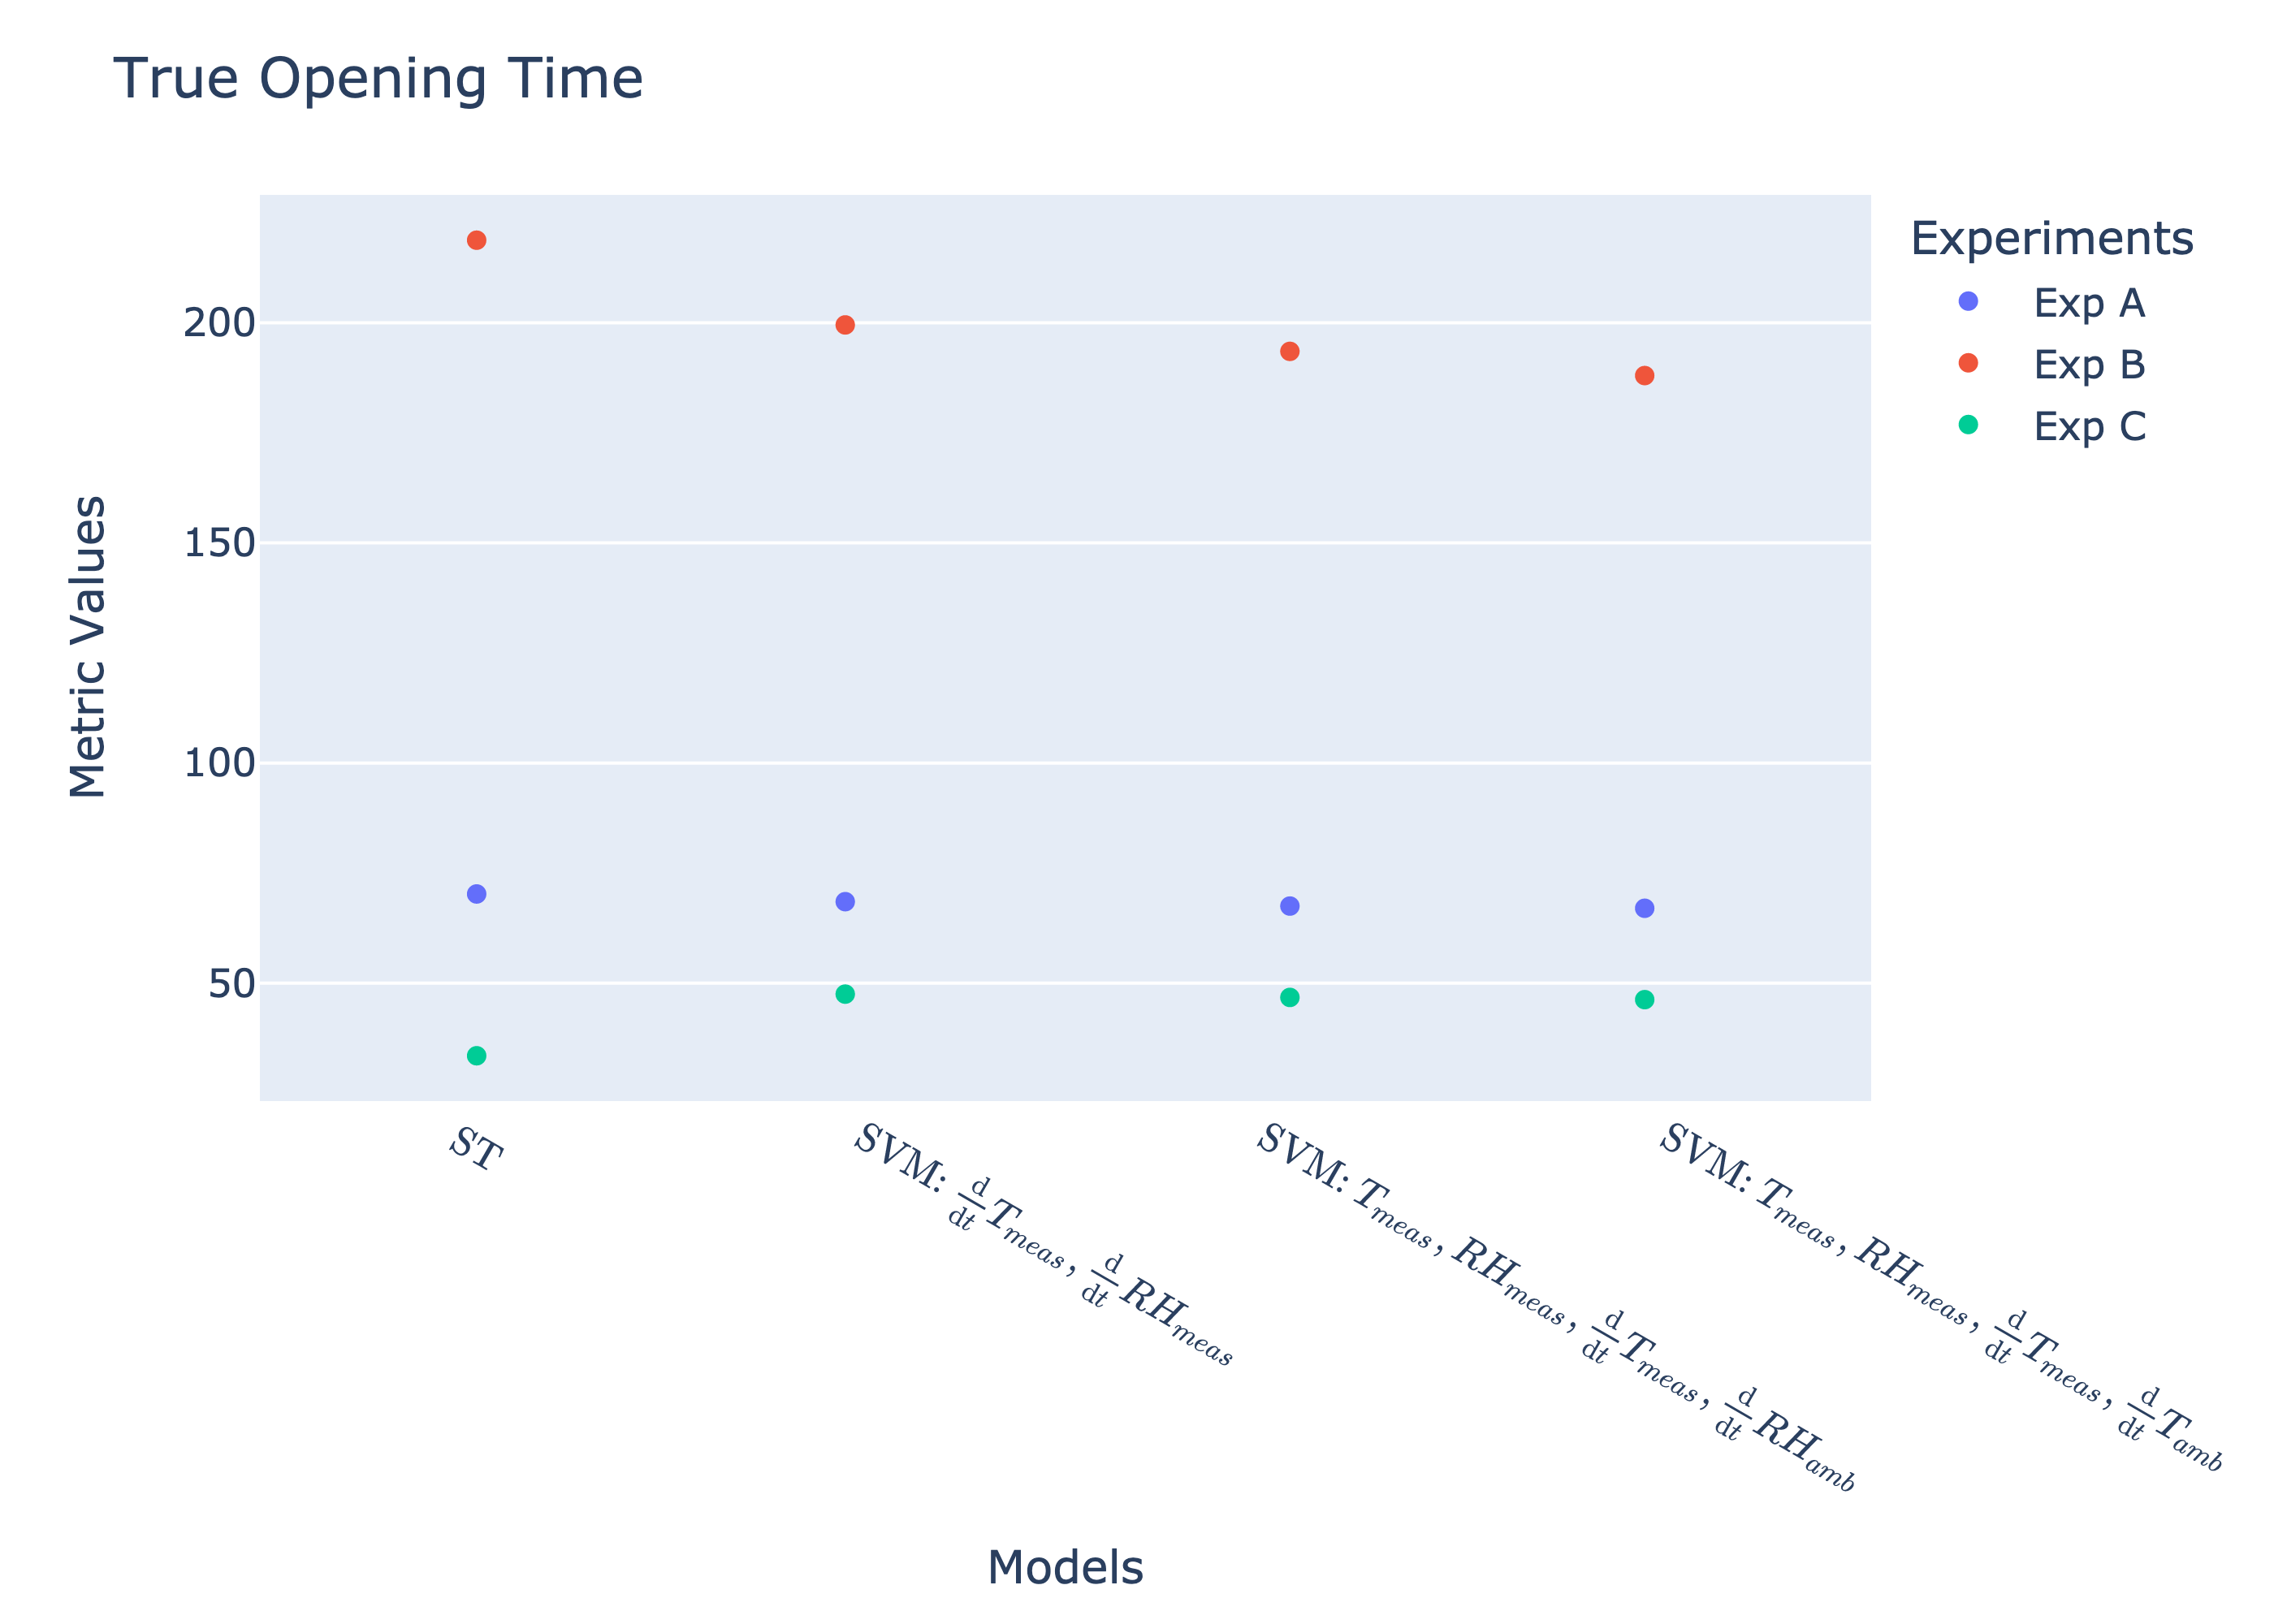
\includegraphics{figs/true_time.png}

}

}

\subcaption{\label{fig-tt}}
\end{minipage}%

\caption{\label{fig-exp-results}Comparison across experiments and
metrics}

\end{figure}

In Figure~\ref{fig-exp-results}, comparisons of ST to the performance of
the SVM across the metrics and datasets are displayed. While ST
represents one model, each of the SVM models shown in each of figures
represents a model that performed unsupervised classification using a
different combination of features. The SVM models are organized
according to performance based on metric, and only the top three models
are shown.

In Figure~\ref{fig-f1}, we see that the ST performs better than the
best-performing SVMs on experiments A and B, but has considerably worse
performance on experiment C. The range of F1-scores displayed in
Figure~\ref{fig-f1} are comparable to those shown in (CITE drdr). The
low values across all models for experiments B and C can be attributed
to the rather unbalanced nature of the datasets, which a macro average
F1-score penalizes.

ST has less accuracy in detecting the ratios of hits to guesses in
experiments B and C compared to the best-performing SVMs, as shown in
Figure~\ref{fig-hg}. However, as Figure~\ref{fig-ga} highlights, the
SVMs take far more guesses per recorded action of window state change,
while ST takes on the order of 1 guess per recorded action. This
suggests that the SVMs' superior performance on the hits over guesses
metric is due to probability, rather than an embedding of the underlying
physical dynamics. (FIX: currently guesses to action is actually showing
worst perfroming SVMs, to make this analysis valid need to sort SVM
based on hits to guess ration)

Figure~\ref{fig-oa} and Figure~\ref{fig-uoa} display the performance on
the opening and unbounded opening accuracy metrics. We observe that ST
has a far higher performance for experiment A, a slightly better
performance for experiment C, and a score of 0 for experiment B. The
unbounded opening accuracy allows us to compare just how ``off'' models
are. We see that ST performs ``less poorly'' than the SVM across all
experiments. This suggests that ST predictions of when window states
change are, on average, closer in time to reality than the predictions
of the SVM models.

The true time and false time metrics, shown in Figure~\ref{fig-tt}
operates as an analog to a weighted average F1-score, in that the the
imbalance between window open and close is inherently taken into
account. ST is true more often and false less often (false opening time
graph not shown) for experiments A and B. The reverse is true for
experiment C.

We see that the ST performs poorly on experiment C, which is the most
unfavorable dataset since it had unbalanced window states and narrow
distinction between indoor and outdoor temperature. Despite poor
performance on this particularly unfavroable dataset, the ST shows
comparable performance to the SVMs across all metrics for the other two
datasets. This finding is significant, given that the SVMs shown in the
graphs have made unsupervised classification decisions a wide range of
combinations of features, and then sorted based on performance to reveal
the optimal feature set for a particular experiment. ST method thus
shows potential as a powerful teqhnique with robust performance across
both favorable and unfavorable datasets.

\hypertarget{conclusions-and-future-work}{%
\section{Conclusions and Future
Work}\label{conclusions-and-future-work}}

We presented preliminary results showcasing the efficacy of a new
method, ST, for unsupervised window detection. We compared these results
with SVM models trained with optimized features, and found comprable
results. Using datasets with notable differences in window state balance
and contrast between indoor and outdoor temperatures enabled us to begin
to test the limits of this new method.

Analyzing a standard metric, the F1-score, as well as the several window
detection specic metrics enabled us to develop a more nuanced
understanding of the nature of the predictions the models made. The
highest performing SVMs for example, tended to detect signifantly more
change points than actually occured in the data. While this behavior can
lead to higher accuracy, it can be harmful for unsupervised detection.
For designing naturally cooled buildings particularly, a practictioner
might want to infer a user's likelihood to use operable windows to
regulate their thermal comfort. The predictions from the SVM models
would suggest that, since windows are frequently being opened or closed,
users are highly engaged with temperature manipulation, when in reality
this is not the case. Therefore, understanding why window detection is
needed, and then creating metrics that respond to this specific use-case
is a key step of unsupervised window state detection.

\hypertarget{future-work}{%
\subsection{Future Work}\label{future-work}}

Although ST has shown promising results, we believe that there are a
number of steps that can be explored for improving its performance.
First, our method does not take into account the material properties of
the room where data is being collected, although this data would be
available from construction documentation. This information could help
to simulate response of indoor quantities of interest to daily seasonal
changes in ambient quantities using simple heat transfer equations. This
would enable us to more precisely identify the seasonal component in
indoor time series which would be an immprovement from the simple
smoothing technique we use here. The addition of momentum equations to
our simulation would enable us examine the magnitude of temperature
change that connvective heat transfer permits when a window is open vs
closed. Understanding expected indoor temperature changes under
different conditions would help to make more educated guesses in the
guessing step of the ST. In summary, augmenting the current data-driven
ST with a better underestanding of the physical processes underlying the
data is a critical next step.

The ST could also possibly be improved carrying out a similar process
for relative humidity as temperature. Features involving relative
humidity featured heavily in the top-performing SVMs, which makes sense,
as indoor relative humidity does have some correlation to ambient
properties. Similar physical simulations as described above could be
carried out to better understand this relationship.

Spatial simulations and measurements could also be helpful in
determining where a sensor should be placed in a room to best capture
the fluctuations in quantities of interest. For this simulation, sensors
were intentionally placed away from from windows so as avoid drafts and
better capture the average temperaure of a space. However, it is
conceivable that sensors placed closer to a window would be more
sensitive to changes in the window state, and thus record a stronger
window change detection signal.

Finally, future work should involve evaluating this method on a wider
variety of datasets. Although the datasets presented here do have
significant differences, they were all collected in adjacent rooms in
the same building. Changing the location where data is collected, and
exploring further ranges of balanced datasets and indoor-outdoor
temperature relationships will be key for validating an unsupervised
model.
\end{document}
